The purpose of this note is to document the plans by the ECCE consortium to re-use the BaBar solenoid.  The BaBar solenoid is currently planned for use in the sPHENIX experiment and will be available after sPHENIX running concludes in 2025. The solenoid provides a 1.4T central field at design current. 

The design parameters of the BaBar solenoid are shown in Figure~\ref{fig:BaBarStats}. 

\begin{figure}[h!tbp]
    \centering
    \includegraphics[width=0.9\textwidth]{figs/BaBar_Stats.png}
    \caption{Parmeters of the BaBar solenoid.}
    \label{fig:BaBarStats}
\end{figure}

\begin{figure}[h!tbp]
    \centering
    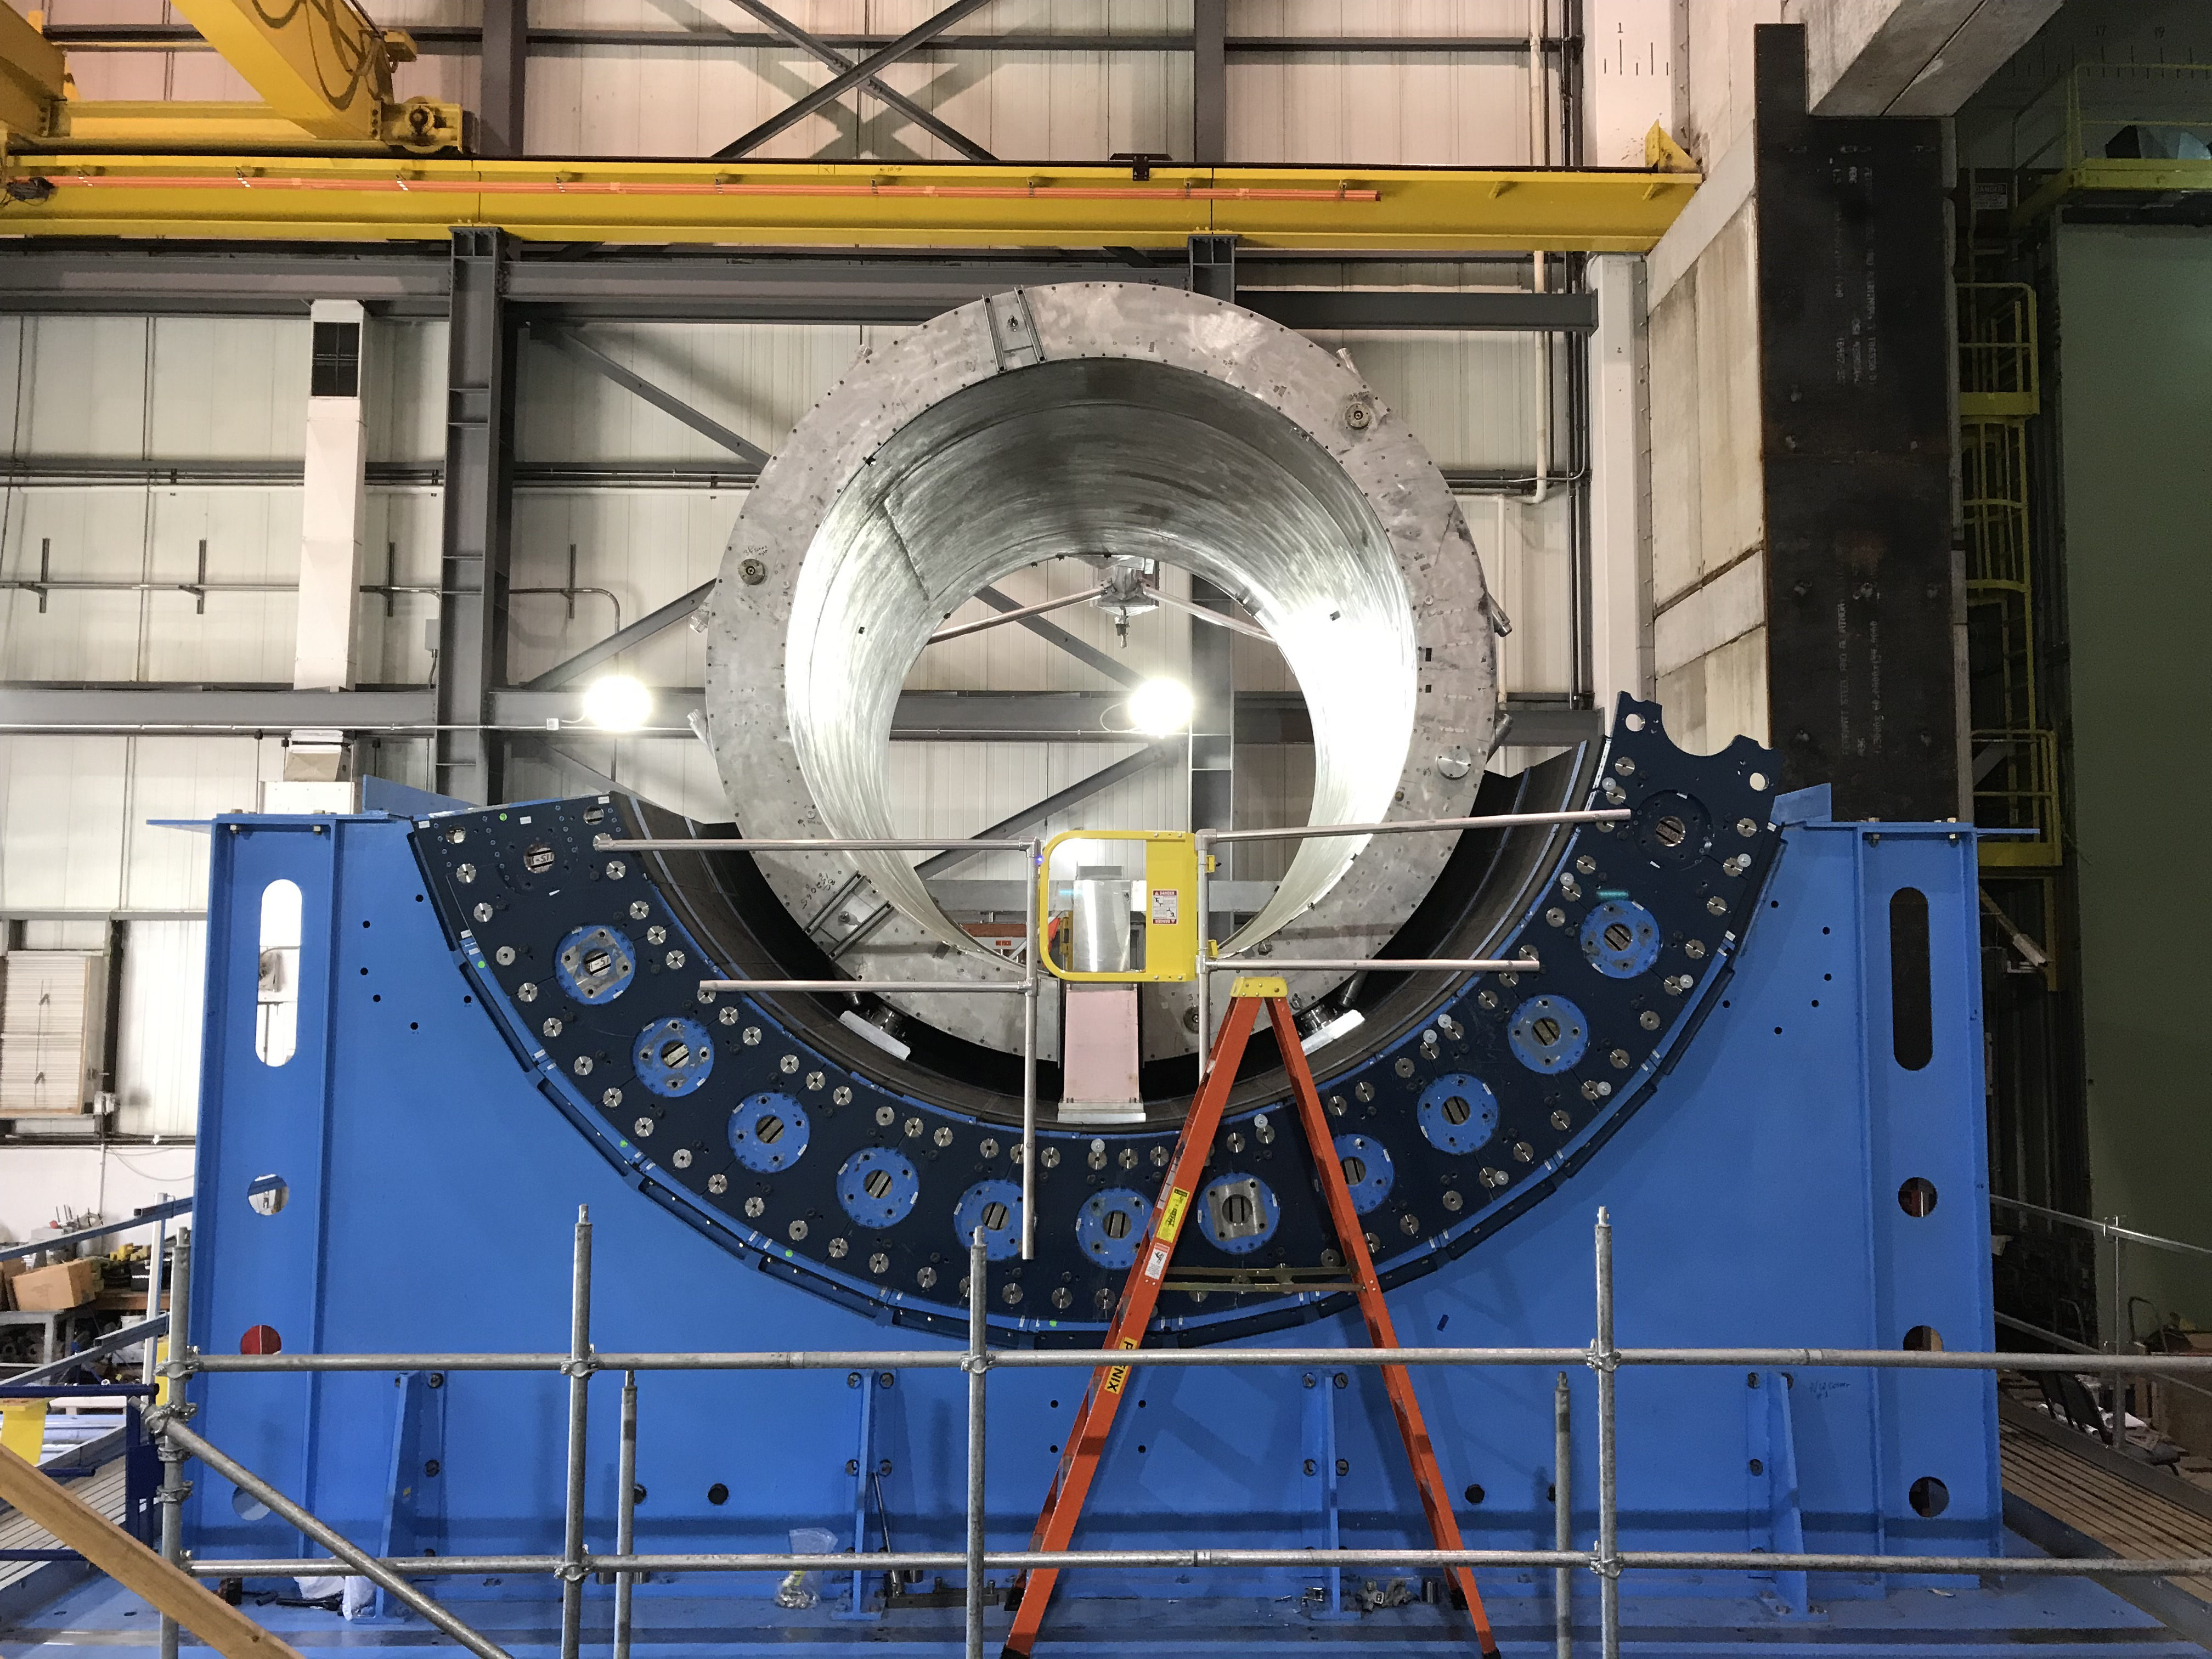
\includegraphics[width=0.9\textwidth]{figs/magnet_install_1.png}
    \caption{The BaBar solenoid in October, 2021, as it was installed in the sPHENIX experiment. The solenoid is resting in the barrel flux return, which will be completed with additional sectors in the coming months.  The experimental cradle, barrel flux return (outer hadronic calorimeter), and BaBar solenoid are all items planned to be re-used by the ECCE experiment.}
    \label{fig:BaBarInSPHENIX}
\end{figure}

\subsection{Refurbishment of the BaBar Solenoid}

The re-use of the magnet has been the subject of a engineering study and risk analysis, available as an EIC Technical Note (EICTJ-O-DE-PLT-TD-0017-R00), which also details the potential actions required to refurbish the BaBar solenoid for use in ECCE. 

After extensive discussions with the JLab engineers, it was decided that any modifications or refurbishment that required opening the BaBar solenoid cryostat would not be worth the additional risk. None of these actions will be necessary if the magnet continues to operate well throughout sPHENIX running. sPHENIX is expected to conduct a high-field magnet test in the experiment flux return (which will also be re-used for ECCE) in mid-2022, followed by experimental operations 2023-25. Figure~\ref{fig:BaBarInSPHENIX} shown the BaBar solenoid installed in the sPHENIX experiment. As a mitigation against the schedule risk posed by a problem with the BaBar solenoid developing late in sPHENIX running, we proceed with the initial engineering and design for a replacement magnet. It is expected a final decision to proceed with the BaBar solenoid or produce a new magnet will be taken in mid-2023 after the performance of the BaBar solenoid during the first year of sPHENIX running is reviewed by a panel of experts.  The risk-mitigation decision tree is shown in Figure~\ref{fig:risk_tree}. 

A draft schedule for the ECCE solenoid is shown in Figure~\ref{fig:magnet_schedule}. 

\begin{figure}[h!tbp]
    \centering
    \includegraphics[width=0.9\textwidth]{figs/flowchart_Page_1.png}
    \caption{Decision tree for the selection of either the ECCE magnet of a new magnet with the same characteristics.}
    \label{fig:risk_tree}
\end{figure}

\begin{sidewaysfigure}[h!tbp]
    \centering
    \includegraphics[width=1.0\textwidth]{figs/ECCE Detector Solenoid_Babar reuse_v5.png}
    \caption{Schedule for the ECCE solenoid.}
    \label{fig:magnet_schedule}
\end{sidewaysfigure}